%
% exemplo genérico de uso da classe iiufrgs.cls
% $Id: iiufrgs.tex,v 1.1.1.1 2005/01/18 23:54:42 avila Exp $
%
% This is an example file and is hereby explicitly put in the
% public domain.
%
\documentclass[cic,tc]{iiufrgs}
% um tipo específico de monografia pode ser informado como parâmetro opcional:
%\documentclass[tese]{iiufrgs}
% monografias em inglês devem receber o parâmetro `english':
%\documentclass[diss,english]{iiufrgs}
% a opção `openright' pode ser usada para forçar inícios de capítulos
% em páginas ímpares
% \documentclass[openright]{iiufrgs}
% para gerar uma versão somente-frente, basta utilizar a opção `oneside':
% \documentclass[oneside]{iiufrgs}
\usepackage[utf8]{inputenc}   % pacote para acentuação
\usepackage{times}              % pacote para usar fonte Adobe Times
\usepackage[alf,abnt-emphasize=bf]{abntex2cite}	% pacote para usar citações abnt
\usepackage{graphicx}          % para inserir imagens
\usepackage{booktabs}
\usepackage{float}     % para as imagens ficarem no lugar certo
%\usepackage{mathptmx}          % p/ usar fonte Adobe Times nas fórmulas

\graphicspath{ {images/} }

\title{Uma análise dos dados de queimada do INPE no Brasil (preliminar)}
\translatedtitle{Using \LaTeX\ to Prepare Documents at II/UFRGS}

\author{Braz}{José Henrique da Silva}
\advisor[Prof.~Dr.]{Schnorr}{Lucas M.}

% a data deve ser a da defesa; se nao especificada, são gerados
% mes e ano correntes
%\date{maio}{2001}

% o nome do curso pode ser redefinido (ex. para TCs)
\course{Curso de Graduação em Ciência da Computação}

% o local de realização do trabalho pode ser especificado (ex. para TCs)
% com o comando \location:
\location{Porto Alegre}{RS}

% palavras-chave
% iniciar todas com letras maiúsculas
%
\keyword{Formatação eletrônica de documentos}
\keyword{\LaTeX}
\keyword{ABNT}
\keyword{UFRGS}

%
% palavras-chave na lingua estrangeira
% iniciar todas com letras maiúsculas
%
\translatedkeyword{Electronic document preparation}
\translatedkeyword{\LaTeX}
\translatedkeyword{ABNT}
\translatedkeyword{UFRGS}

%
% inicio do documento
%
\begin{document}

% folha de rosto
% às vezes é necessário redefinir algum comando logo antes de produzir
% a folha de rosto:
% \renewcommand{\coordname}{Coordenadora do Curso}
\maketitle

% dedicatoria
\clearpage
\begin{flushright}
\mbox{}\vfill
{\sffamily\itshape
``If I have seen farther than others,\\
it is because I stood on the shoulders of giants.''\\}
--- \textsc{Sir~Isaac Newton}
\end{flushright}

% agradecimentos
\chapter*{Agradecimentos}
Agradeço ao \LaTeX\ por não ter vírus de macro\ldots

% sumario
\tableofcontents

% lista de abreviaturas e siglas
% o parametro deve ser a abreviatura mais longa
% A NBR 14724:2011 estipula que a ordem das abreviações
% na lista deve ser alfabética (como no exemplo abaixo).
\begin{listofabbrv}{SPMD}
	\item[API] Application Programming Interface (Interface de Programação de Aplicação)
	\item[CSV] Comma Separated Values (valores separados por vírgulas).
    \item[GMT] Greenwich Mean Time
    \item[INPE] Instituto Nacional de Pesquisas Espaciais
    \item[IBGE] Instituto Brasileiro de Geografia e Estatística
    \item[URL] Uniform Resource Locator (Localizador Uniforme de Recursos)
    \item[NOAA] National Oceanic and Atmosphere Administration
    \item[MODIS] Moderate Resolution Imaging Spectroradiometer
    \item[GOES] Geostationary Operational Environmental Satellite
    \item[AVHRR] Advanced Very High Resolution Radiometer
\end{listofabbrv}

% idem para a lista de símbolos
%\begin{listofsymbols}{$\alpha\beta\pi\omega$}
%       \item[$\sum{\frac{a}{b}}$] Somatório do produtório
%       \item[$\alpha\beta\pi\omega$] Fator de inconstância do resultado
%\end{listofsymbols}

% lista de figuras
\listoffigures

% lista de tabelas
\listoftables

% resumo na língua do documento
\begin{abstract}
Este documento é um exemplo de como formatar documentos para o
Instituto de Informática da UFRGS usando as classes \LaTeX\
disponibilizadas pelo UTUG\@. Ao mesmo tempo, pode servir de consulta
para comandos mais genéricos. \emph{O texto do resumo não deve
conter mais do que 500 palavras.}
\end{abstract}

% resumo na outra língua
\begin{translatedabstract}
This document is an example on how to prepare documents at II/UFRGS
using the \LaTeX\ classes provided by the UTUG\@. At the same time, it
may serve as a guide for general-purpose commands. \emph{The text in
the abstract should not contain more than 500~words.}
\end{translatedabstract}

% aqui comeca o texto propriamente dito

%%%%%%%%%%%%%%%%%%%%%%%%%%%%%%%%%%%%%%%%%%%%%%%%%%%%%%%%%%%%%%%%%%%%%%%%%%%%%%%

\chapter{Introdução}

O fogo é uma tecnologia que está presente há milênios no território que hoje é o Brasil, desde queimadas controladas pelo povo indígena Kayapó no cerrado para plantio ou caça, até incêndios iniciados por combustão espontânea em períodos de seca no sul da Amazônia. O uso do fogo pelos indígenas era controlado, levando em conta o clima atual e a vegetação a ser queimada, e restrito apenas a um período do ano, com o intuito de reduzir pragas e ajudar nas plantações \citep{leonel_2000}. [P0. O que é uma queimada/fogo] \par

Hoje as queimadas que mais chamam atenção estão diretamente ligadas ao processo de desmatamento e manejo de áreas agrícolas para o cultivo da monocultura de soja. O fogo também é a prática mais barata e rápida para limpar áreas inteiras para a pecuária bovina. Commodites agrícolas e carne bovina movem a economia do Brasil, que é o maior exportador desses produtos, e aumentam a pressão para o desmatamento de novas áreas na Amazônia \citep{fuchs_2020}. [P1. As queimadas hoje] \par

O Brasil ocupa a quarta posição no ranking de nações que mais emitem gases de efeito estufa por habitantes, segundo dados da United Nations Environment Programme (UNEP) de 2022. De acordo com o estudo, o valor absoluto se manteve estável desde 2010, e atingiu seu pico por volta dos anos de 2003 a 2004. Assim como a Indonésia, o que melhor explica a alta posição do Brasil neste ranking são as queimadas e o desmatamento da vegetação nativa. Olhando para os municípios do país, dos dez que mais poluem, oito deles estão localizados no bioma da amazônia e não possuem atividades industriais que justificariam esse valor. [P2. queimadas e efeito estufa no Brasil] \par

\begin{figure}[H]
    \caption{Emissões de gases do efeito estufa per capta de 1990 até 2020 (tCO2e/capita).}
    \begin{center}
        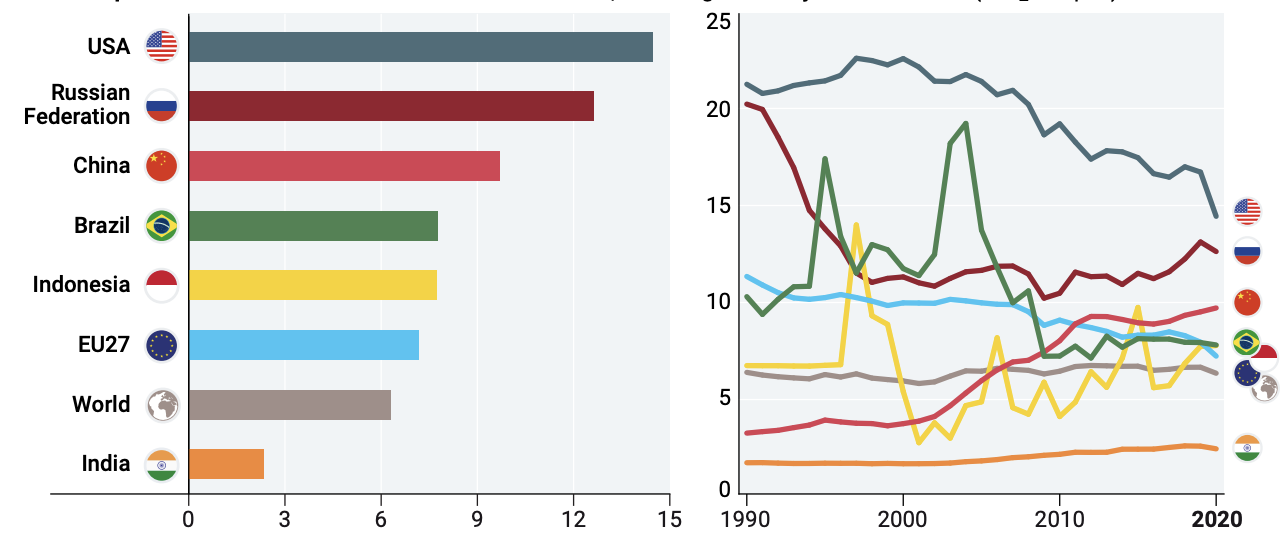
\includegraphics[width=35em]{emissoes_gee_per_capta}
    \end{center}
    \legend{Fonte: Emissions Gap Report 2022: The Closing Window}
    \label{fig:emissoes_gee_per_capta}
\end{figure}

Este trabalho se dedica a estudar e apresentar de forma concisa os dados de focos de queimadas disponibilizados pelo Instituto Nacional de Pesquisas Espaciais (INPE). O principal objetivo é tornar fácil o entendimento desses dados gerados a partir de imagens de satélites, sem a necessidade de um conhecimento prévio das técnicas de ciência de dados e sensoriamento remoto. O escopo de tempo das análises é limitado ao início de 1998, ano que iniciou a base aberta de queimadas, até o final de 2022. [P3. O que é o trabalho em si] \par

Os dados analisados neste trabalho foram obtidos a partir do DBQueimadas, Banco de Dados de Queimadas \url{www.inpe.br/queimadas/bdqueimadas}, que é um sistema desenvolvido pelo INPE e acessível de forma aberta por meio da web. Conta com mais de 300 milhões de pontos coletados desde o ano de 1998, provenientes de vários satélites \citep{setzer2019banco}. Ao disponibilizar os dados das queimadas o instituto possibilita que a sociedade retribua com pesquisas e fomenta novas abordagens ao problema das queimadas no Brasil, como é o caso deste trabalho. [P4. Fonte dos dados usados] \par

... apontaram que a detecção de áreas queimadas pode se beneficiar da fusão de observações de incêndios ativos de vários sensores. \citep{giglio2010assessing} ........ mas incendios ativos podem ficar omissos \citep{giglio2009active} ....... \par

Durante o decorrer do documento são apresentadas diversas figuras, a maioria de construção do próprio autor, a fim de instigar a intuição do leitor para o tópico que está sendo abordado. De início, será abordado questões mais teóricas envolvendo caracteríscas dos satélites, suas produções de imagens e como são usadas para detectar um foco ativo de queimada. Após isso, .... [P5. Estrutura do documento] \par


%%%%%%%%%%%%%%%%%%%%%%%%%%%%%%%%%%%%%%%%%%%%%%%%%%%%%%%%%%%%%%%%%%%%%%%%%%%%%%%

\chapter{Conceitos básicos e visão geral dos dados}

Neste capítulo, serão apresentados conceitos importantes para a compreensão do trabalho. Primeiramente, serão formalizadas definições relacionadas às queimadas e à forma como são monitoradas no Brasil. Em seguida, será realizada uma sumarização dos principais satélites utilizados pelo INPE e suas características. Além disso, será abordado como as imagens geradas pelos satélites são utilizadas para a detecção de focos ativos. Por fim, apresentaremos uma análise dos dados para demonstrar uma visão geral das principais tendências e gráficos. \par

\section{O monitoramento das queimadas no Brasil}

Um foco de queima, também conhecido como "Fire Pixel", é a detecção de fogo na vegetação em uma área correspondente ao tamanho de um pixel na imagem gerada pelo satélite. Um incêndio pode durar dias e queimar uma grande extensão de terra, o que provavelmente resultará na detecção de vários focos de queima a partir das imagens dos satélites. O número de focos de queima está diretamente relacionado à extensão total queimada e pode ser utilizado para comparações e análises. No entanto, é importante destacar que o foco de queima por si só não representa de forma precisa o que está acontecendo na região, mas é um indicador valioso da intensidade e extensão do fogo. \par


[P0. Diferença entre foco detectado e área queimada] \par

[P1. Falar um pouco do INPE e suas divisões] \par

Dentro do site é possível gerar mapas, tabelas, gráficos e exportar os dados sobre as queimadas no Brasil aplicando diferentes filtros. Todo o programa foi desenvolvido com ferramentas abertas, muitas delas criadas pelo próprio time de tecnologia da informação do INPE \citep{setzer2019banco}. \par

O Banco de Dados de Queimadas é um excelente caso de como os dados abertos podem ajudar a sociedade. Além do DBQueimadas, o INPE também disponibiliza para visualização e download, por meio da Divisão de Geração de Imagens (DGI) \url{www.dgi.inpe.br/catalogo/}, algumas imagens inteiras geradas pelos satélites que o próprio DGI captura e processa. \par

Para obter as imagens brutas dos satélites são necessárias antenas especiais que ficam em centros de recepção de dados. Com esse propósito, a DGI possui duas Estações de Recepção e Gravação (ERG) - a primeira em Cachoeira Paulista (SP) e uma mais recente em Cuiabá (MT). Na estação de SP, é feito o processamento de mais de 200 imagens de diversos satélites todos os dias, extraindo os dados de focos ativos de queimadas que alimentam o DBQueimadas \citep{SiteDGI}. \par

É em posse dessas imagens brutas que o INPE aplica algoritmos de detecção de focos de queimadas, abordado na Sessão \ref{sec:deteccao_focos_section}. No caso da detecção ser positiva, a posição exata (latitude e longitude) e a hora que a imagem foi gerada são adicionadas aos dados como uma nova linha e disponibilizados pelo DBQueimadas. O INPE ainda coloca junto com as coordenadas da detecção mais alguns dados como risco de fogo, poder do fogo, precipitação e dados referentes a região do foco. A lista completa das colunas pode ser vista na Tabela \ref{table:inpeColumns} \cite{PerguntasFrequentesINPE}. \par

\begin{table}[htbp]
\centering
\caption{Significado de cada coluna dos dados de queimada do INPE.}
\begin{tabular}{@{}llp{9cm}@{}}
 \toprule
 \texttt{Atributo} & \texttt{Tipo} & Descrição \\
 \midrule
 \texttt{Id} & \texttt{string} & Identificador único registrado no banco \\
 \texttt{Latitude} & \texttt{double} & Graus decimais da latitude do centro 
                     do pixel de fogo ativo (valores de 90.0000 até -90.0000) \\ 
 \texttt{Longitude} & \texttt{double} & Graus decimais da longitude do centro 
                     do pixel de fogo ativo (valores de 180.0000 até -180.0000) \\  
 \texttt{DataHora} & \texttt{string} & Data a hora da passagem do satélite no fuso 
                     horário de Greenwich (GMT) \\   
 \texttt{Municipio} & \texttt{string} & Nome do município, de acordo com os dados 
                     do IBGE 2000 \\
 \texttt{Estado} & \texttt{string} & Nome do estado \\
 \texttt{Pais} & \texttt{string} & Nome do país \\  
 \texttt{Bioma} & \texttt{string} & Nome do bioma brasileiro, de acordo com 
                     dados do IBGE 2004 (para outros países o campo fica vazio) \\
 \texttt{Precipitação} & \texttt{double} & Valor a precipitação do dia até 
                     o horário da medida (-999 para valores inválidos) \\
 \texttt{DiasSCh} & \texttt{integer} & Dias sem chuva até a data da medida 
                     (-999 para valores inválidos) \\
 \texttt{RiscoFog} & \texttt{double} & Valor do risco de fogo previsto naquele dia 
                     (-999 para valores inválidos) \\
 \texttt{FRP} & \texttt{double} & Fire Radiative Power, MW (megawatts) \\
 \bottomrule
\end{tabular}
\legend{Fonte: O Autor com base em \citet{PerguntasFrequentesINPE}}
\label{table:inpeColumns}
\end{table}

\section{Os Satélites}

O INPE processa atualmente dados de diversos satélites, cada um com características distintas. Esses satélites abrangem uma ampla gama de órbitas e altitudes, desde satélites geoestacionários, como o GOES-12, localizado a 29.400 km de distância da superfície \citep{GOES12Algo}, até satélites em órbitas polares, que ficam entre 700 e 900 km de altura. Cada um desses satélites é equipado com diferentes sensores que são utilizados para diversos propósitos, como observação da vegetação terrestre, nuvens, oceanos e monitoramento atmosférico. \par

Cada satélite pode estar equipado com um sensor imageador que captura imagens com características distintas. Esses sensores são capazes de captar não apenas a luz visível, no intervalo de 400 nm a 700 nm, mas também o infravermelho, de 780 nm a 1 mm. As medições realizadas pelos sensores são divididas em canais, que diferem em termos de resolução espacial - a escala geográfica representada por cada pixel da imagem - e resolução espectral, ou seja, o intervalo de comprimento de onda abrangido. Geralmente, o primeiro canal é dedicado à luz visível, abrangendo o espectro do laranja ao vermelho e possui a maior resolução espacial possível para o sensor. Os demais canais utilizam diferentes intervalos de comprimento de onda do infravermelho e da luz visível, frequentemente com incremento na resolução espacial. \par

Os satélites também podem ser classificados de acordo com o tipo de óbita, que pode ser polar ou geoestacionária. Os satélites polares percorrem toda a terra, com uma altitude baixa e alta velocidade, passando várias vezes pelos polos norte e sul em um único dia. Já os satélites geoestacionários ajustam sua orbita para sempre parecerem estacionários em relação a um ponto fixo na Terra. Esses satélites ficam em altitudes mais altas devido à sua velocidade mais baixa, que é igual à rotação da Terra. A Figura \ref{fig:orbita2022-08-10}, gerada a partir de dados do site Celestrak (\url{https://celestrak.org/}), mostra a passagem de alguns satélites polares no Brasil no dia 10 de agosto de 2022. Também é possível ver o satélite geoestacioário GOES-16, localizado ao norte do perú, representado com um ponto no gráfico. \par

\begin{figure}[H]
    \caption{Órbita dos satélites no dia 10 de agosto de 2022.}
    \begin{center}
        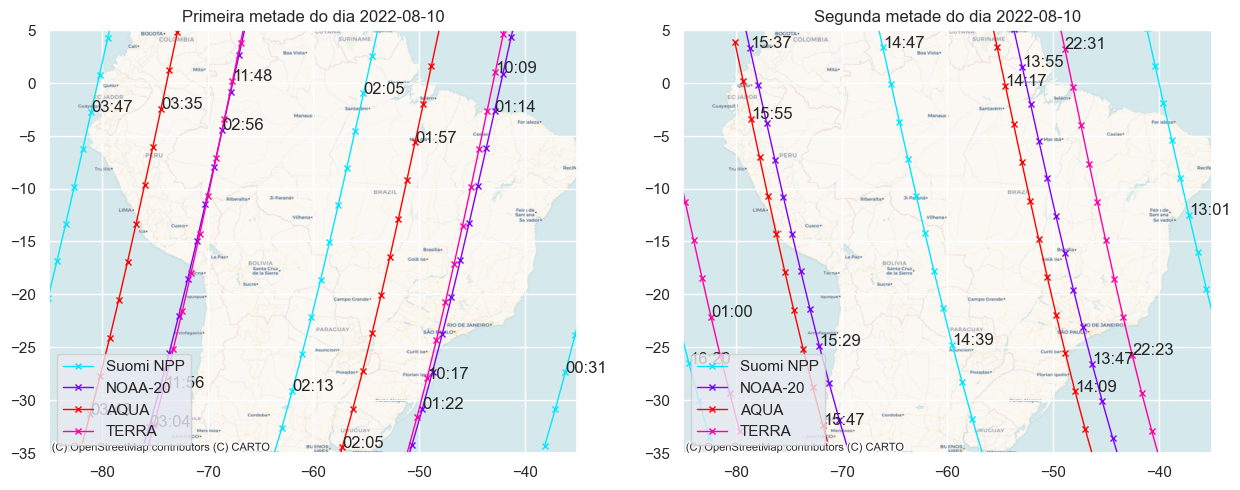
\includegraphics[width=35em]{orbita2022-08-10}
    \end{center}
    \legend{Fonte: O Autor}
    \label{fig:orbita2022-08-10}
\end{figure}

A Tabela \ref{table:satelites} contém um resumo dos satélites utilizados pelo INPE desde o início da série histórica até o final de 2022 \cite{EmbrapaSatelites}. Atualmente, os satélites que estão em pleno funcionamento são: NOAA-20, NOAA-19, NOAA-18, GOES-16, Suomi NPP, AQUA, TERRA, MSG-03, METOP-B e METOP-C. Os demais satélites, como NOAA-17, NOAA-16, NOAA-15, TRMM, NOAA-14, NOAA-12, GOES-13, MSG-02, GOES-12, GOES-10 e GOES-08, deixaram de operar em diferentes momentos devido a problemas técnicos ou ao fim de sua vida útil e componentes. \par

\begin{table}[htbp]
\centering
\caption{Características dos satélites usados pelo INPE.}
\begin{tabular}{ @{}llllcl@{} }
  \toprule
  Nome    & Sensor & Resolução esp. & Órbita & Lançamento & Passagem \\
  \midrule
  METOP-C & AVHRR-3  & 1100m       & Polar   & 2018 & 21h \\
  NOAA-20 & VIIRS    & 500m        & Polar   & 2017 & 2h / 14h \\
  METOP-B & AVHRR-3  & 1100m       & Polar   & 2012 & 21h \\
  Suomi NPP & VIIRS  & 500m        & Polar   & 2011 & 2h / 14h \\
  NOAA-19 & AVHRR-3  & 1100m       & Polar   & 2009 & 2h / 14h \\
  NOAA-18 & AVHRR-3  & 1100m       & Polar   & 2005 & Variadas \\
  AQUA    & MODIS    & 1000m       & Polar   & 2002 & 2h / 14h \\
  NOAA-17 & AVHRR-3  & 1100m       & Polar   & 2002 & 21h \\
  NOAA-16 & AVHRR-3  & 1100m       & Polar   & 2000 & Variadas \\
  TERRA   & MODIS    & 1000m       & Polar   & 1999 & 11h / 23h \\
  NOAA-15 & AVHRR-3  & 1100m       & Polar   & 1998 & 5h / 17h \\
  TRMM    & VIRS     & 2000m       & Polar   & 1997 & Variadas \\
  ERS-2   & ATSR-2   & 1000m       & Polar   & 1995 & Variadas \\
  NOAA-14 & AVHRR    & 1100m       & Polar   & 1994 & 21h \\
  NOAA-12 & AVHRR    & 1100m       & Polar   & 1991 & 2h / 15h \\
  ERS-1   & ATSR-1   & 1000m       & Polar   & 1991 & Variadas \\
  GOES-16 & ABI      & 2000m       & Geoest. & 2016 & Não se aplica \\
  MSG-03  & SEVIRI   & 3000m       & Geoest. & 2012 & Não se aplica \\
  GOES-13 & GOES I-M & 4000m       & Geoest. & 2006 & Não se aplica \\
  MSG-02  & SEVIRI   & 3000m       & Geoest. & 2005 & Não se aplica \\
  GOES-12 & GOES I-M & 4000m       & Geoest. & 2001 & Não se aplica \\
  GOES-10 & GOES I-M & 4000m       & Geoest. & 1997 & Não se aplica \\
  GOES-08 & GOES I-M & 4000m       & Geoest. & 1994 & Não se aplica \\
  \bottomrule
\end{tabular}
\legend{Fonte: O Autor com base em \citet{EmbrapaSatelites}}
\label{table:satelites}
\end{table}

Os satélites TERRA e AQUA, ambos com o sensor Moderate Resolution Imaging Spectroradiometer (MODIS), foram lançados em 1999 e 2002 respectivamente. São americanos e foram desenvolvidos em parceria com o Japão, Canada e Brasil. O sensor MODIS possui 36 canais e resolução espectral que varia de 250m a 1km em diferentes espectros do infravermelo e luz visível. É especialmente capaz de detectar mudanças no uso e cobertura da terra bem como queimadas e atividades vulcânicas. \par

Os satélites da série NOAA (National Oceanic and Atmospheric Administration) são operados pela agência americana de mesmo nome. Embora tenha havido vários satélites NOAA ao longo do tempo, atualmente estão em operação o NOAA-20, NOAA-19 e NOAA-18. Esses satélites desempenham um papel fundamental no fornecimento de dados para a previsão do tempo e o monitoramento da vegetação. 

Além dos satélites NOAA, em 2011, a NOAA em parceria com a NASA lançou o satélite Suomi NPP (Suomi National Polar-orbiting Partnership). O Suomi NPP tem como objetivo principal obter observações ambientais e meteorológicas avançadas da Terra. É equipado com o sensor VIIRS (Visible Infrared Imaging Radiometer Suite), que também está presente no NOAA-20. Esses dois satélites, Suomi NPP e NOAA-20, são os satélites com mais alta resolução espacial entre todos os processados pelo INPE. \par 

O conjunto de satélites GOES (Geostationary Operational Environmental Satellite) é operado pela NASA e controlado também pelo NOAA. As primeiras versões desses satélites geoestacionários foram equipadas com o sensor GOES I-M (Imager Radiometer e Vertical Sounder) de resolução espacial equivalente a 4km. A partir do GOES-16 o sensor foi substituído pelo ABI (Advanced Baseline Imager), capaz de produzir imagens com resolução 4 vezes melhores. Esse conjunto de satélites foi e ainda é muito usado nas previsões metereológicas nos países do continente americano. \par

O INPE processa as imagens dos satélites da série METOP (Meteorological Operational Satellite), incluindo o METOP-B e o METOP-C, bem como os satélites da série MSG (Meteosat Second Generation), como o MSG-02 (Meteosat-9) e o MSG-03 (Meteosat-10). Ambas missões projetadas em parceria com a ESA (Agência Espacial Europeia) e a EUMETSAT (Organização Europeia para a Exploração de Satélites Meteorológicos). Esses satélites têm como objetivo a previsão do tempo, o monitoramento climático e o acompanhamento de desastres naturais. O METOP-C é o último satélite planejado para a série METOP, completando assim o conjunto de satélites METOP-A, METOP-B e METOP-C.

O instituto também processou dados dos satélites ERS-1 e ERS-2, equipados com o sensor ATRS (Along Track Scanning Radiometer) da Agência Espacial Europeia (ESA) \cite{EmbrapaSatelites}. Esses satélites, de órbita polar, são especializados em medir com precisão a temperatura da terra e dos oceanos. Os dados coletados por esses satélites são utilizados por cientistas para detectar mudanças climáticas e vegetação, incluindo eventos como queimadas, em todo o planeta. O ATRS possui duas versões, sendo que o primeiro (ATSR-1) possui 4 canais e o segundo (ATSR-2) foi aprimorado com um canal adicional para capturar a luz visível, possibilitando o monitoramento da vegetação.  \par

Também estão presentes nos dados, em menor escala, os focos de queimadas obtidos pelo satélite TRMM (Tropical Rainfall Measuring Mission). O TRMM foi uma missão conjunta entre a NASA e a JAXA (Agência Espacial Japonesa), que teve início em 1997 e oficialmente encerrou em 2015. O principal objetivo dessa missão era estudar a distribuição de chuvas e tempestades, bem como suas influências no clima global. \par

Para estabelecer uma série temporal consistente e permitir a análise de tendências ao longo de vários anos dos focos de queimadas detectados em diferentes regiões, o INPE definiu um satélite de referência. Esse satélite de referência é escolhido com base em critérios específicos. É importante que sua órbita cubra satisfatoriamente a área do país, sem distorcer os dados de forma significativa. Além disso, é desejável que os sensores do satélite tenham resoluções adequadas, ou seja, não muito baixas, para garantir uma análise precisa dos focos de queimadas.

No período de 01 de junho de 1998 a 03 de julho de 2002, o satélite de referência utilizado foi o NOAA-12, com passagem no final da tarde. Após esse período, passou-se a utilizar o satélite AQUA, com passagem à tarde (identificado nos dados como AQUA\_M-T). O AQUA tem operado além da data prevista de encerramento e provavelmente deve ser descontinuado em breve. Quando isso ocorrer, a previsão é que o satélite Suomi NPP deve ser o novo satélite de referência \citep{PerguntasFrequentesINPE}. Sempre que há uma mudança de satélite de referência, a série histórica de quantidade de focos de queimada precisa ser ajustada devido a diferença entre os satélites.

\section{Detecção de focos de queimadas e área queimada}
\label{sec:deteccao_focos_section}

O algoritmo para identificação de focos ativos a partir de imagens de satélites é específico para cada tipo de sensor. No geral, eles usam diferentes canais dos sensores dos satélites, entre a luz visível e o infravermelho, e podem ter comportamentos distintos dependendo se a imagem foi gerada à noite ou de dia. Podem também usar limiares dinâmicos, de acordo com a região do planeta, que são calculados com base em uma espécie de média das temperaturas nas regiões próximas ao longo dos dias. Além disso, é comum a aplicação de máscaras para eliminar regiões submersas, costeiras, deserticas e que estavam nubladas na hora da passagem. \par

Para o caso dos satélites TERRA e AQUA, que têm o sensor MODIS, o instituto mantinha seu próprio método de detecção, que produzia dados de maior confiabilidade \citep{PerguntasFrequentesINPE}. A partir de 2017 o INPE migrou toda a base de dados para o "Collection 6", algoritmo aplicado pela \textit{National Aeronautics and Space Administration} (NASA), marcando o início da chamada Base 2 de queimadas. Anteriormente, a NASA empregava o Collection 5, que gerava falsos positivos em clareiras florestais e falsos negativos para grandes queimadas obscurecidas por fumaça densa.\citep{SCHROEDER2008}. [P3. Algoritmo empregrado pelo INPE] \par

O collection 6 .... \citep{GIGLIO2016} \par

Para detectar áreas queimadas, o instituto atualmente usa o produto AQ1km, desenvolvido em parceria com o Laboratório de Aplicações de Satélites Ambientais (LASA) \citep{SiteAQ1km} que ainda está em fase Provisória (ainda pode sofrer mudanças e não foi validada completamente). O produto é aplicados nos dados do sensor MODIS e, desta forma, usa os satélites AQUA e TERRA de forma concomitante \citep{libonati2015algorithm}. Uma vez que o AQUA foi lançado apenas em 2002, o produto só pode ser usados para dados a partir de 2003. \par

O AQ1km .... \citep{libonati2015algorithm} \par

\section{Uma visão geral dos dados}

Nesta sessão, será realizada uma análise inicial dos dados disponíveis sobre focos de queimada, com o objetivo de extrair algumas informações relevantes. É importante, no entanto, ter cuidado na escolha dos satélites a serem utilizados na análise. Para algumas análises, caso sejam usados todos os satélites disponíveis, pode ocorrer a contagem de um mesmo foco várias vezes ou, ainda, a contagem do mesmo foco em passagens diurnas e noturnas de um mesmo satélite polar. Para solucionar esse problema, será utilizado o satélite AQUA com passagem à tarde (AQUA\_M-T), que é  o satélite de referência do INPE atualmente. Dessa forma, é possível evitar a contagem duplicada de focos de queimada e garantir a precisão das informações analisadas. \par

Com relação aos satélites, e possível perceber a partir da Figura \ref{fig:porcentagem_satelites} cinco satélites que mais identificaram focos de queimada em toda a série história, são eles: Suomi NPP, GOES-16, AQUA, NOAA-16 e TERRA. Todos eles estão ativos atualmente e com quantidades de coleta significativas em 2022. AQUA e TERRA são os mais antigos e possuem um sensor obsoleto. O GOES-16 é um satélite geoestacionário, conhecido por gerar dados de forma mais frequente, geralmente detecta apenas queimadas maiores devido a sua posição distante da Terra. Suomi NPP e NOAA-20 possuem um sensor que detecta 10 vezes mais focos que sensor MODIS. Por estar em atividade a mais tempo, o Suomi NPP gerou mais dados que o NOAA-20. \par

\begin{figure}[H]
    \caption{Relação do montante dos dados por satélite.}
    \begin{center}
        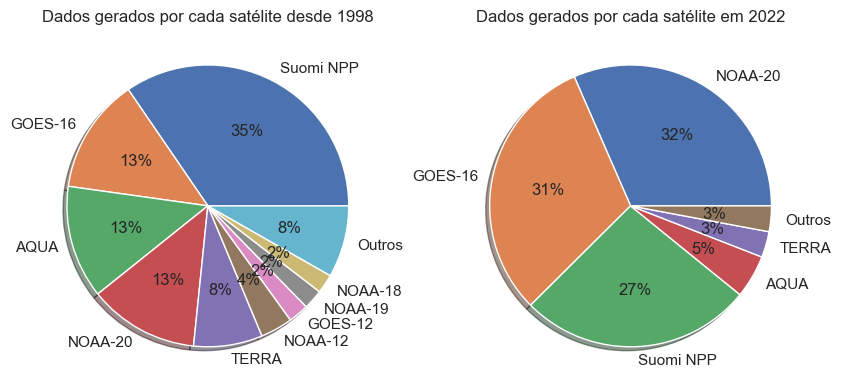
\includegraphics[width=35em]{porcentagem_satelites}
    \end{center}
    \legend{Fonte: O Autor}
    \label{fig:porcentagem_satelites}
\end{figure}

Saber em quais momentos os satélites passam também é importante para a análise. Os satélites polares passam duas vezes por dia no Brasil, variando o local exato da passagem de acordo com as características de sua órbita. Pela Figura \ref{fig:tempo_medidas_satelites} é possível observar esse comportamento empiricamente, em que as 5 primeiras linhas, que representam dados gerados por satélites polares, apresentam dois picos durante um período de 24 horas. Já para o  caso dos geoestacionários (GOES-16), que ficam fixos em relação a uma posição na Terra, não se observou o mesmo padrão. \par

\begin{figure}[H]
    \caption{Amostragem por tempo de cada satélite.}
    \begin{center}
        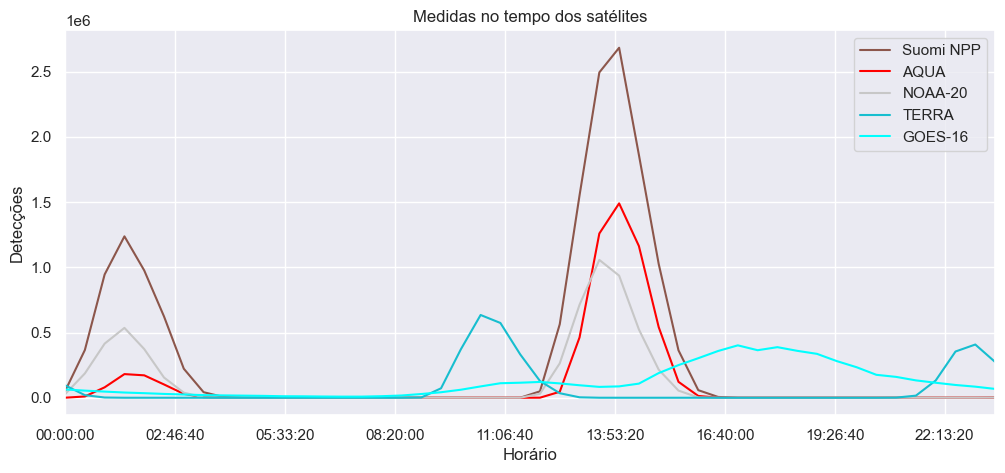
\includegraphics[width=35em]{tempo_medidas_satelites}
    \end{center}
    \legend{Fonte: O Autor}
    \label{fig:tempo_medidas_satelites}
\end{figure}

A partir de uma análise quantitativa dos dados com relação ao tempo de cada medida, exposto na Figura \ref{fig:quantitativo_geral}, podemos identificar uma grande sazonalidade, sempre tendo picos entre os meses de agosto e setembro. Desde o início da série, o mês que mais teve focos detectados foi setembro de 2007. 

\begin{figure}[H]
    \caption{}
    \begin{center}
        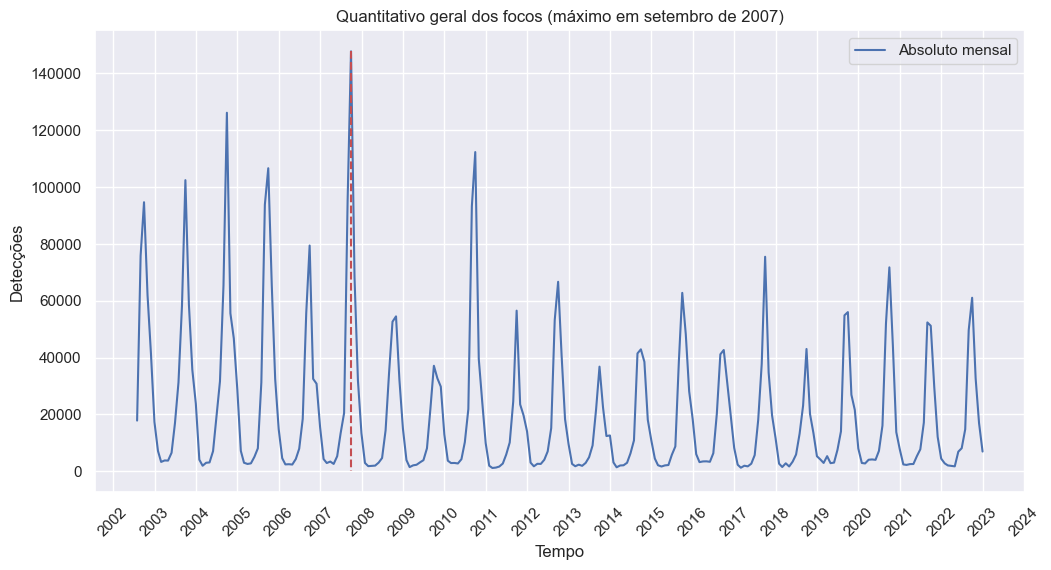
\includegraphics[width=35em]{quantitativo_geral}
    \end{center}
    \legend{Fonte: O Autor}
    \label{fig:quantitativo_geral}
\end{figure}


P1. Fazer análise preliminar dos dados gerando alguns gráficos \par
P2. Gráficos geral do brasil com os focos de queimadas totais \cite{geographicDataSciencePython} \par


%%%%%%%%%%%%%%%%%%%%%%%%%%%%%%%%%%%%%%%%%%%%%%%%%%%%%%%%%%%%%%%%%%%%%%%%%%%%%%%

\chapter{Trabalhos Relacionados}
\label{chp:trabalhos_relacionados}

Muitos outros trabalhos antes deste versaram sobre os dados de queimadas do INPE e, em menor escala, especicamente sobre o cálculo das áreas queimadas. Nesse capítulo, serão apresentado alguns trabalhos que estão de alguma forma próximos deste e, no final, será discutido o que faz este de certa forma único. \par

O primeiro estudo refere-se ao trabalho que embasou o produto AQ1km \citep{libonati2015algorithm}, desenvolvido pelo INPE. O objetivo do estudo é detectar áreas queimadas mensalmente por meio de sensoriamento remoto utilizando o sensor MODIS (satélites AQUA e TERRA). Para isso, o algoritmo identifica regiões que apresentaram fogo ativo usando diferentes satélites, extraídos da mesma base do INPE, e agrupa os dados a cada um mês. Em seguida, filtra essas regiões com base em um índice de vegetação sensível a queimadas no espectro do infravermelho próximo, em relação ao mesmo índice do mês anterior. Por fim, identifica regiões próximas às regiões classificadas como área queimada no passo anterior, mas que não apresentaram um indicador forte o suficiente, o que pode ser devido a uma queimada parcial ou baixa intensidade de fogo naquele local. \par



%%%%%%%%%%%%%%%%%%%%%%%%%%%%%%%%%%%%%%%%%%%%%%%%%%%%%%%%%%%%%%%%%%%%%%%%%%%%%%%


\chapter{Metodologia}

Neste capítulo será abordado como método utilizado para calcular as áreas queimadas foi desenvolvido. Começa com uma visão geral do método, depois entra em cada etapa de forma separada e mais detalhada.

\section{Visão geral da metodologia}

A metodologia desenvolvida visa calcular a área de vegetação queimada no Brasil, por meio da análise dos dados de focos de queimadas disponibilizados pelo INPE, juntamente com as características dos diferentes satélites e sensores. A premissa fundamental é que um foco de queimada detectado resulta em uma área queimada. Além disso, considera-se que a quantidade de focos detectados em uma determinada região, em um intervalo de tempo, está diretamente relacionada com a área efetivamente queimada na região. \par 

\begin{figure}[H]
    \caption{Diagrama do método. A entrada principal são os dados de focos de queimadas e a saída principal é a estimativa de áreas queimadas. Abaixo os resultados produzidos com a aplicação em um determinado local para cada estapa.}
    \begin{center}
        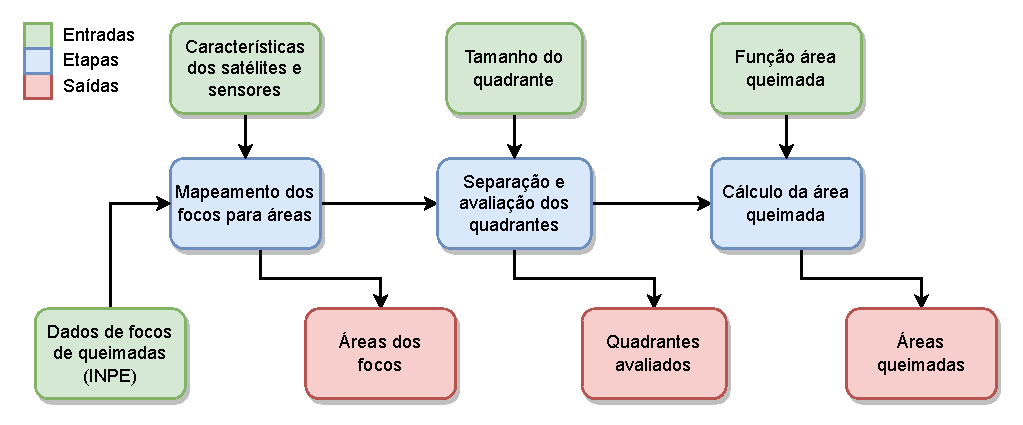
\includegraphics[width=35em]{metodologica_workflow}
        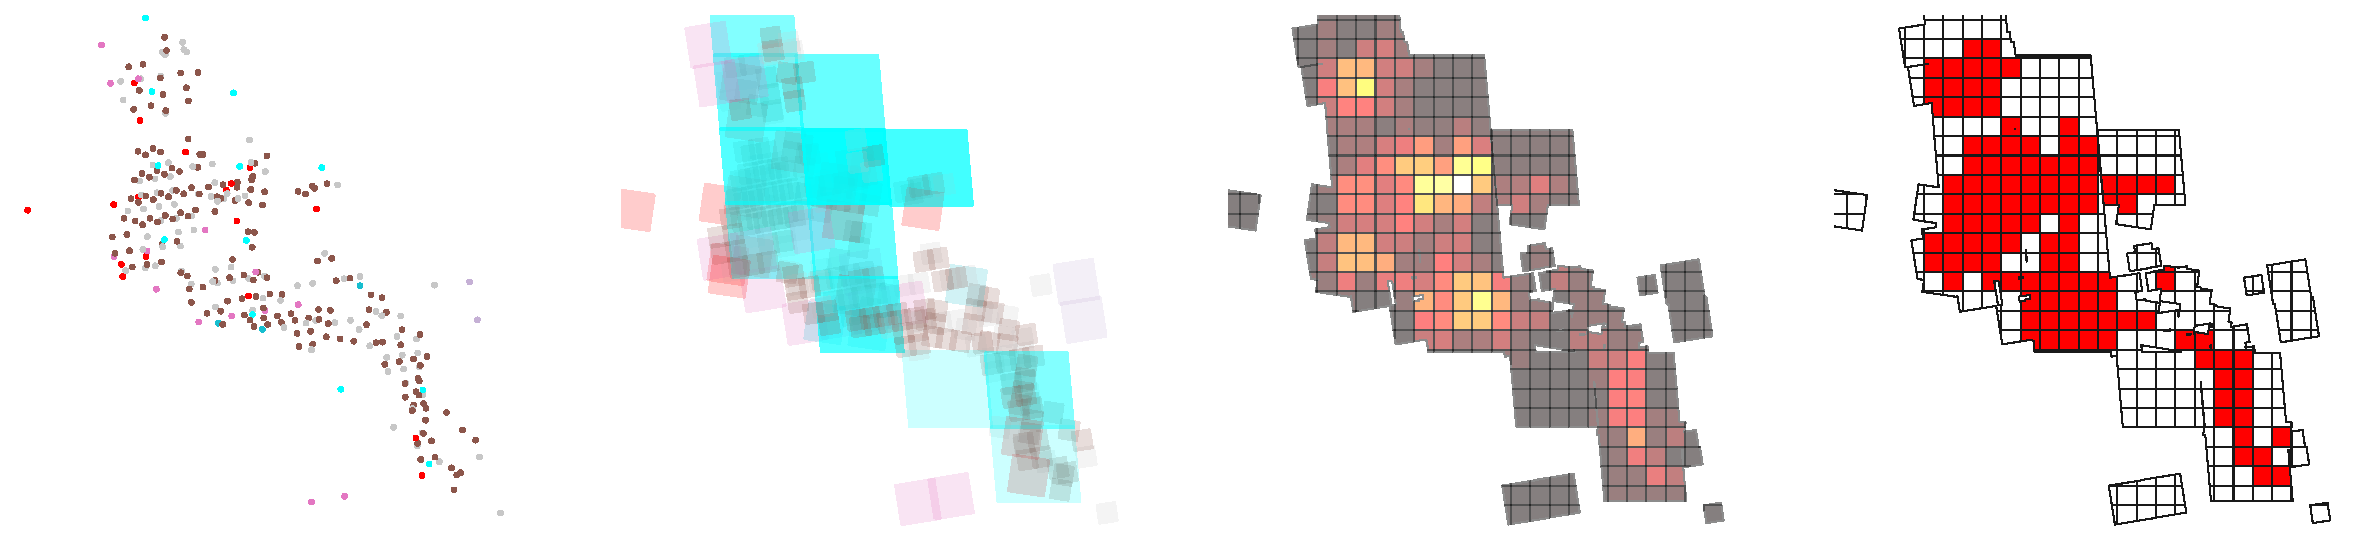
\includegraphics[width=35em]{exemplo_metodo_completo}
    \end{center}
    \legend{Fonte: O Autor}
    \label{fig:metodologica_workflow}
\end{figure}

O método completo, conforme apresentado na Figura \ref{fig:metodologica_workflow}, é composto por três principais etapas (cartões em azul): mapeamento dos focos para áreas, separação e avaliação dos quadrantes, e cálculo da área queimada. Cada etapa recebe dados de entrada e produz uma saída que, com exceção da última etapa, é usada como entrada para a etapa subsequente.

A primeira etapa transforma os pontos dos focos em áreas que representam a abrangência do foco. Essa etapa recebe dados de focos de queimadas do INPE, previamente filtrados para o intervalo de tempo de interesse, e produz como saída as áreas de cada foco. Essas áreas estão diretamente relacionadas às características do satélite e sensor que captaram a imagem original, como abordado em \ref{sec:deteccao_focos_section}, e, portanto, também precisam ser uma entrada para essa etapa.

Na segunda etapa, o espaço é dividido em quadrantes e avaliado. Esse passo recebe as áreas dos focos calculados na etapa anterior e o tamanho do quadrante, que pode ser definido pelo pesquisador. A saída são quadrantes com valores que representam a intensidade das queimadas ocorridas dentro de cada quadrante específico. A função de avaliação é proporcional à diversidade e quantidade das áreas de foco que interceptam os quadrantes.

Na terceira e última etapa, é realizado o cálculo das áreas queimadas, produzindo o resultado final do método. Essa etapa recebe como entrada os quadrantes avaliados no passo anterior e uma função de avaliação da área queimada, que pode ser definida pelo pesquisador. A função é aplicada a todos os quadrantes, resultando em um valor que representa a porcentagem provável de que a área do quadrante tenha sido queimada.

A Figura \ref{fig:metodologica_workflow} também ilustra a aplicação completa do método em uma área específica localizada no sudoeste do Pará, durante os dias 1 a 3 de setembro de 2022. Na primeira imagem, são mostrados os focos de queimada, sem nenhum tipo de pré-processamento. Na segunda imagem, os pontos são transformados em áreas. Em seguida, o espaço é dividido em quadrantes e avaliados. Na última imagem, o cálculo da área queimada considera todas as avaliações acima do valor 5 como quadrante totalmente queimado, resultando em uma área queimada de $33,32 km^2$.

O método é flexível e altamente configurável, podendo assim gerar resultados bem diferentes dependendo de suas entradas, ainda que para o mesmo conjunto de dados de focos. O pesquisador pode testar combinações de entradas e avaliar os resultados usando algum comparador (benchmark). Um exemplo seria compara as saídas do método com os resultado obtidos pelo produto AQ1km (abordado no capítulo \ref{chp:trabalhos_relacionados}). Por fim, a aplicação do método bem como os resultados obtidos são abordados no capítulo \ref{chp:resultados_discussão}.

\section{Mapeamento dos focos para áreas}

Quando um foco de queimada é detectado pelo INPE a partir de um satélite, o foco representa uma área quadrada aproximadamente do tamanho da resolução do sensor que capturou a imagem original. Ou seja, um foco dectado a partir de imagens do satélite AQUA, que utiliza o sensor MODIS, representa uma área de $\approx1Km^2$. Para um satélite com o sensor menos preciso, como o GOES-13, que utiliza o sensor GOES I-M com resolução espacial de $4Km$, a área representada seria 16 vezes maior, indicando uma menor precisão. \par

O cálculo exato da área coberta pelo foco deve levar em conta, além da resolução do sensor, as distorções provenientes dos seguintes fatores: Diferença de localização entre o foco e o satélite, e as caractísticas da órbita do satélite. No primeiro fator, quanto maior a distância entre os dois pontos, maior será a distorção em relação a área de corbertura do sensor. Para um satélite geoestacionário, por exemplo, essa distância é sempre muito grande, devido a sua órbita com altura de $36Km$ \citep{EmbrapaSatelites}. \par

No segundo fator, a inclinação dos satélites determinam como é a rotação da área coberta. Os satélites que orbitam a Terra em órbitas polares, possuem uma determinada inclinação que lhes permitem cobrir diferentes áreas de todo o planeta durante sua tragetória (Figura \ref{fig:orbita2022-08-10}). Quando o satélite está se movendo em uma trajetória ascendente, ou seja, do sul para o norte, a área coberta pelo sensor deve ser rotacionada em um sentido. Por outro lado, se a trajetória for descendente, do norte para o sul, a rotação deve ser no outro sentido. \par

\begin{figure}[H]
    \caption{Comparação entre pontos e áreas dos focos detectados pelo satélite Suomi NPP.}
    \begin{center}
        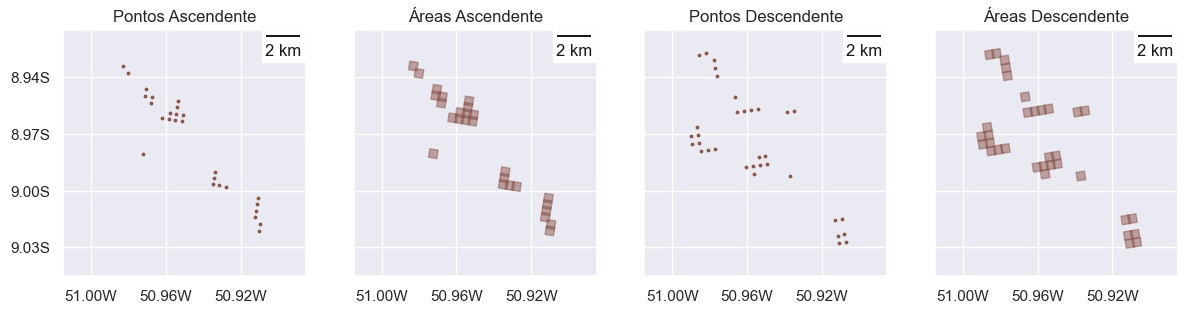
\includegraphics[width=35em]{comparacao_pontos_e_areas}
    \end{center}
    \legend{Fonte: O Autor}
    \label{fig:comparacao_pontos_e_areas}
\end{figure}

A Figura \ref{fig:comparacao_pontos_e_areas} apresenta dados coletados pelo satélite  Suomi NPP no dia dois de setembro de 2022. O primeiro par de imagens corresponde à órbita ascendente do satélite, enquanto o segundo par de imagens corresponde à órbita descendente. Observa-se que, na primeira e terceira imagens, os pontos dos focos de queimada estão alinhados, mas ligeiramente rotacionados em alguns graus, coincidindo com a inclinação do satélite. Na segunda e quarta imagens, os pontos ganham a área do sensor ($500m$) e encaixam perfeitamente entre seus vizinhos. A partir desse ponto até o final do documento, a área coberta pelo foco será chamada de medição. \par

\section{Separação e avaliação de quadrantes}

A separação entre quadrantes é a forma de discretizar os dados do espaço, que são contínuos. Os quadrantes abstraem os detalhes das medições dos diferentes satélites, com diferentes áreas e orientações. Como resultado, ilustrado na figura \ref{fig:satellite_quads_split}, temos uma grade regular que é usado para as operações de avaliação de serão descritas a seguir. \par

O tamanho do quadrante é uma entrada dessa etapa e pode ser definida pelo pesquisador. O valor recomendado desta entrada fica em torno de 0,004 a 0,005 graus, o que coincide com o tamanho da menor resolução de sensor presente nos dados, que é o VIIRS de 500m. \par

\begin{figure}[H]
    \caption{Separação entre quadrantes.}
    \begin{center}
        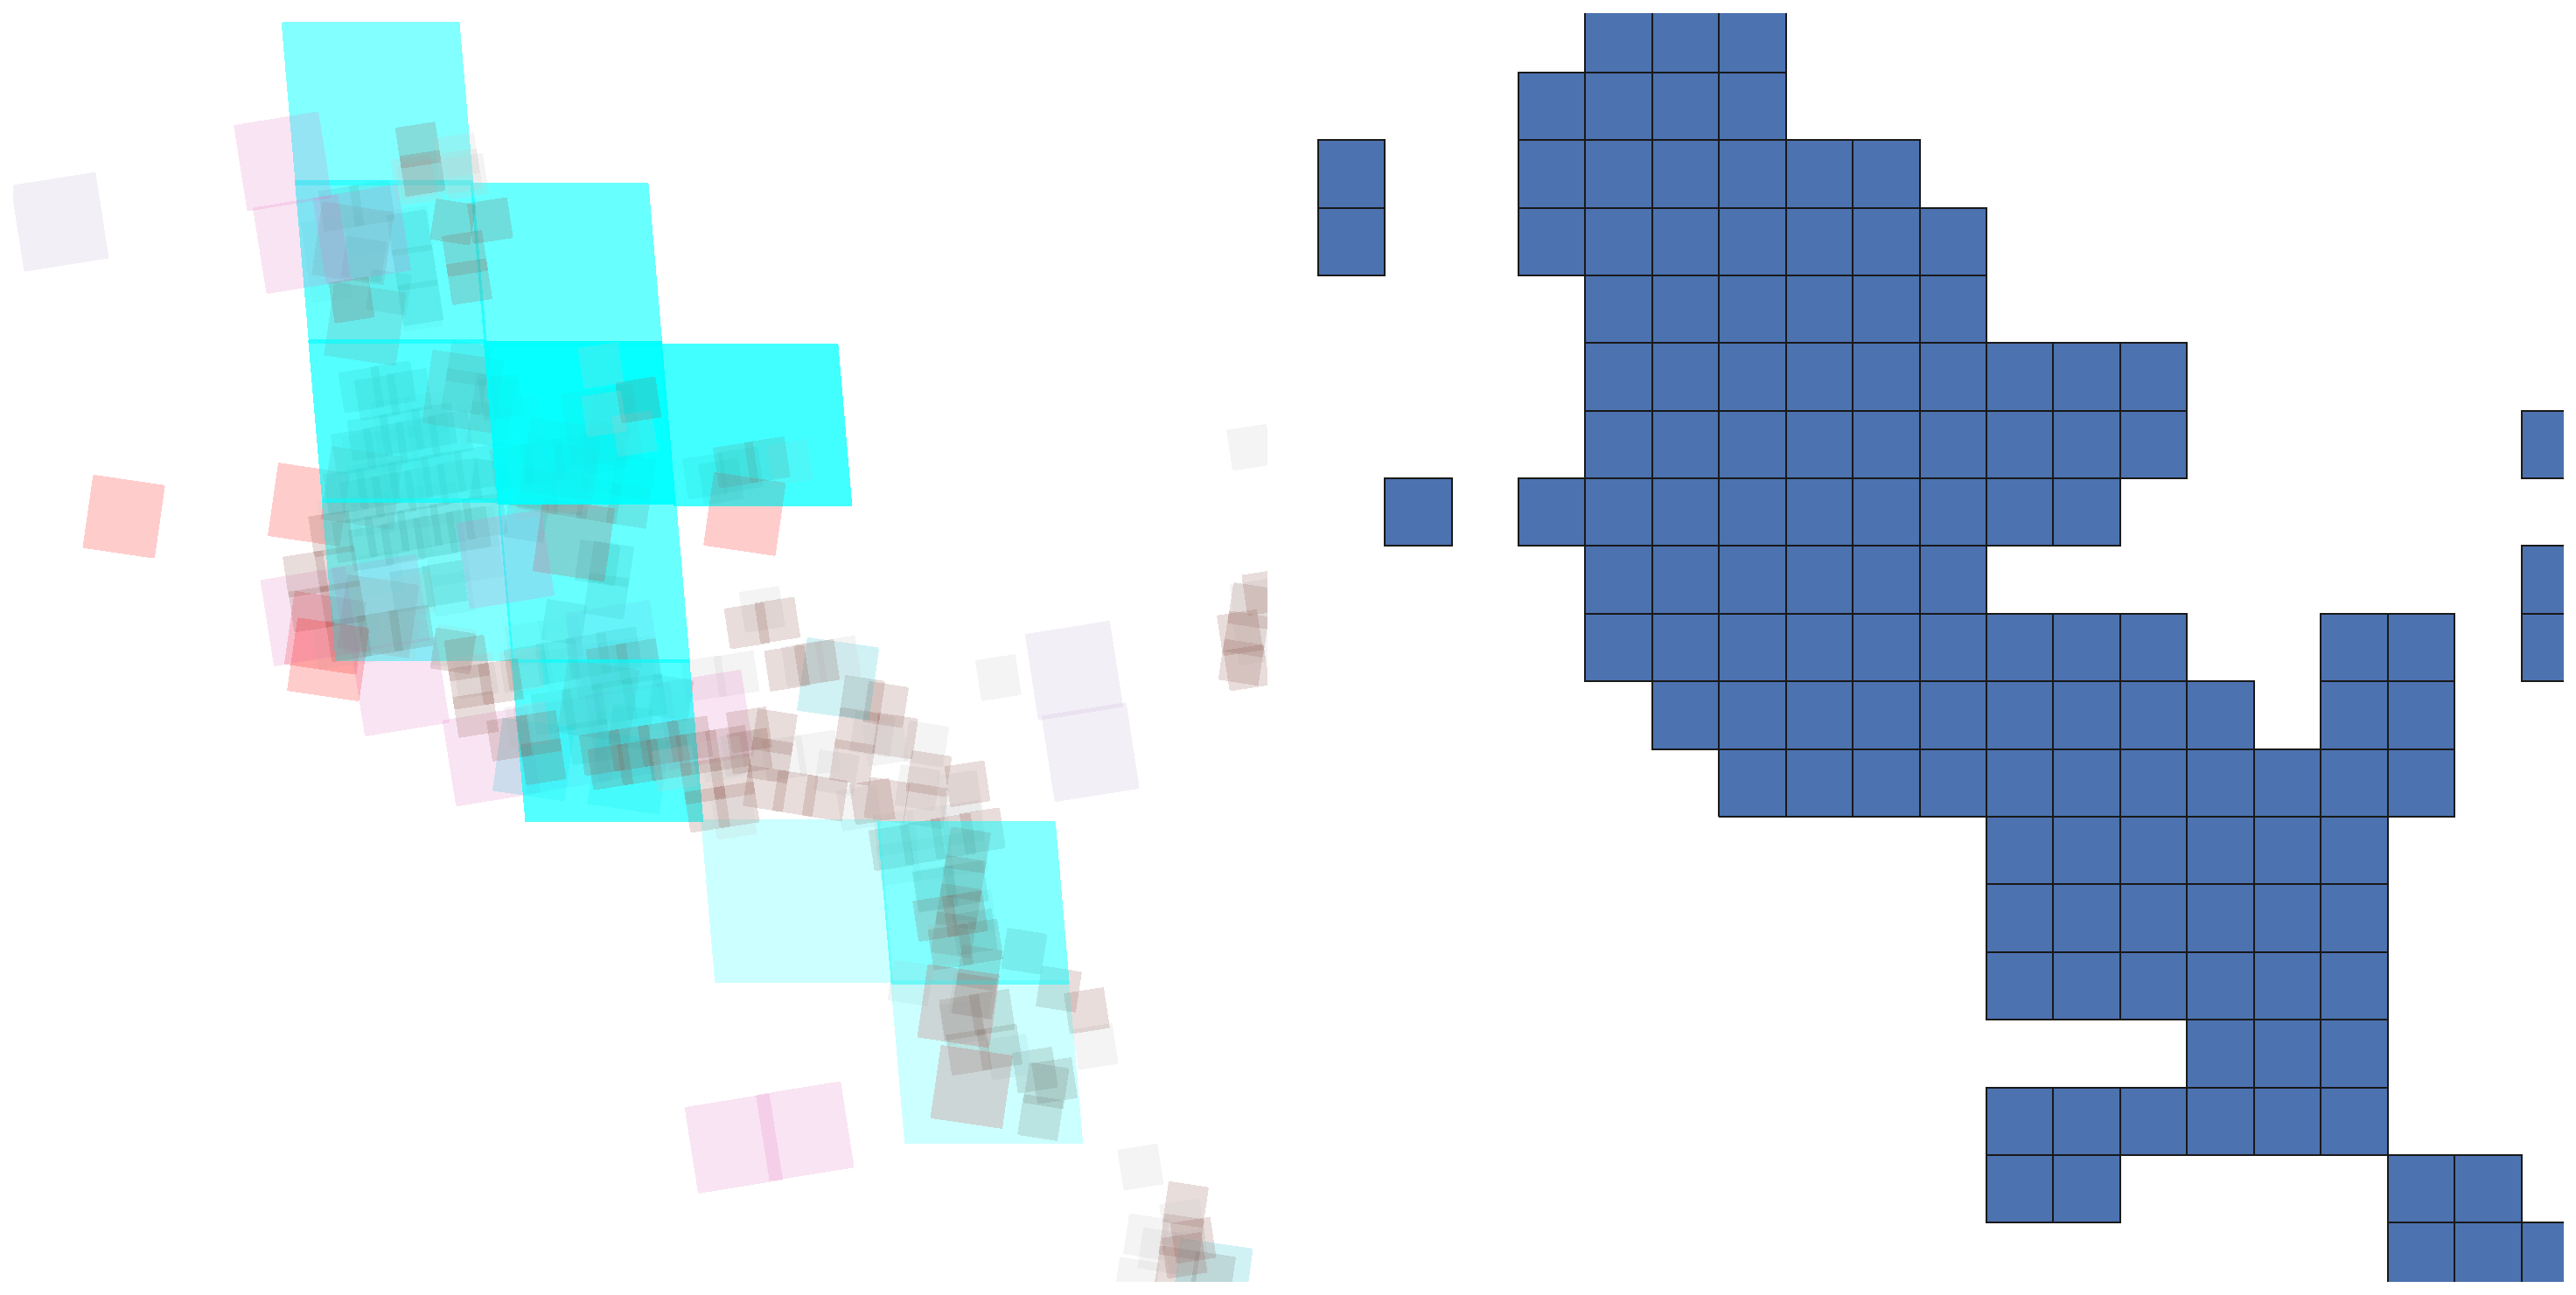
\includegraphics[width=20em]{satellite_quads_split}
    \end{center}
    \legend{Fonte: O Autor}
    \label{fig:satellite_quads_split}
\end{figure}

Com a distribuição dos quadrantes definida, é necessário atribuir a cada um deles um valor que represente a probabilidade de que a área contida tenha sido queimada. A avaliação dos quadrantes deve valorizar aqueles que apresentam medições de diferentes satélites. Essa abordagem justifica-se pelo fato de que ajuda a reduzir os ruídos nas medições e a identificar queimadas mais intensas. Além disso, diferentes satélites realizam medições em horários distintos (veja a Figura \ref{fig:tempo_medidas_satelites}), o que indica uma queimada mais prolongada. Em ambos os casos, queimadas mais intensas e duradouras sinalizam um maior potencial de o fogo se espalhar para outras áreas da vegetação. \par

Sendo $q$ o quadrante (polígono) a ser avaliado; $M$ um conjunto de todas as medições (área coberta pelo foco); operação $area(p)$ retorna a área de um polígono $p$ qualquer; operação $unique\_satelite(Q)$ retorna todos os satélites diferentes do conjunto $Q$; $min\_area$ é a área mínima de uma medição; $threshold\_satellite$ é o número mínimo de satélites para não ser penalizado. A definição formal da avaliação é dada por: \par

Para cada quadrante ($q$), é realizado o cálculo da intersecção com cada medição ($m$) contida nele, resultando em um conjunto $Qm$: \par

\begin{equation} \label{eqn:def_qm}
Qm = \{ m \in M \mid m \cap q \}
\end{equation}

Em seguida, é realizada uma filtragem no conjunto $Qm$, removendo todos os elementos que não possuem uma determinada área mínima, resultando em $Qm'$: \par

\begin{equation} \label{eqn:def_qm_line}
Qm' = \{ m \in Qm \mid area\left(m\right) \ge min\_area \}
\end{equation}

A partir de $Qm'$, é extraído o número de satélites diferentes presentes nesse conjunto, que é denominado $Us$: \par

\begin{equation} \label{eqn:def_us}
Us = \{ m \in unique\_satelite\left(Qm'\right) \}
\end{equation}

Além disso, é calculada a soma das áreas de $Qm'$ e dividida pela área total de $q$, resultando em $ia$. Ou seja, quantas vezes as áreas de $Qm'$ cabem dentro de $q$: \par

\begin{equation} \label{eqn:def_ia}
ia = \left(\sum_{m}^{Qm'} area\left(m\right)\right) \div area(q)
\end{equation}

Penalização de quadrantes que tenham poucos satélites diferentes, o valor de $c$ fica entre 0 e 1 e é linear. \par

\begin{equation} \label{eqn:def_c}
c = 1 - min\left(1, \frac{|Us|}{threshold\_satellite}\right)
\end{equation}

Finalmente, a avaliação final do quadrante ($aq$) é obtida pela expressão: \par

\begin{equation} \label{eqn:def_aq}
aq = |Us|^2 + ia - ai \cdot c
\end{equation}

A fórmula final \ref{eqn:def_aq} atribui um peso quadrático à quantidade de satélites diferentes presente no quadrante $q$. Isso garante que, à medida que a diversidade de satélites aumenta dentro do quadrante, o valor de $aq$ aumente de forma exponencial e se distaque dos demais quadrantes com menos diversidade. O resultado é somado com $ai$, que representa quantas vezes a área das medições somadas cabe no quadrante $q$. Esse termo impede que medições com pouca interseção dentro do quadrante tenham uma influência desproporcional no resultado final. \par

Além disso, há uma penalização aplicada aos quadrantes que apresentam poucos satélites diferentes. Quando a quantidade de satélites diferentes em um quadrante é maior do que um limite pré-estabelecido, chamado de $threshold\_satellite$, não há penalizações, ou seja, o valor de $c$ é igual a 0. Por outro lado, quando o quadrante não atinge o limite, uma parcela de $ai$ é descontada do resultado final. \par

Essa etapa é considerada concluída quando todos os quadrantes estão avaliados seguindo as equações apresentadas. Desta forma, a avaliação de um quadrante não depende de outras avaliações de seus vizinhos ou outra forma de dependência de dados, o que possibilita a avaliação paralela dos quadrantes. \par

\section{Cálculo da área queimada}

Finalmente, com os quadrantes avaliados, é possível estimar a área queimada para cada quadrante. É importante que o método de cálculo seja flexível, permitindo que o pesquisador teste diferentes métodos. Uma forma de fazer isso é atribuir um número que represente a porcentagem de área queimada dentro do quadrante e, em seguida, multiplicá-lo pela área total do quadrante para obter a área queimada dentro do quadrante. Após calcular a área queimada de cada quadrante, é necessário somar todos esses valores para obter a área total queimada. \par

Nesse sentido, o papel do pesquisador é definir uma função ($eval(v)$) que receba o valor do quadrante, calculado na etapa anterior, e retorne um número real entre zero e um. Essa função também pode receber o maior e o menor valor presente na avaliação dos quadrantes, valores que podem ser usados para normalizar o cálculo. Ou seja, o pesquisador pode definir uma função linear que indique que o quadrante só deve ser considerado totalmente queimado se o valor do quadrante for o maior.\par

Para facilitar o trabalho do pesquisador, a implementação pode fornecer funções embutidas comuns que definem a função $eval(v)$. Na Figura \ref{fig:eval_func_built_in}, são apresentadas algumas possibilidades de definições para essa função. A função mais simples é chamada de limiar, que estabelece que toda a área do quadrante deve ser considerada queimada se a avaliação for maior que um determinado valor e nenhuma área deve ser considerada queimada se não alcançar esse valor. Outra função simples é a linear, que faz o valor da área queimada crescer de forma linear dentro de um valor máximo e mínimo. A última função é a exponencial, semelhante à linear, mas com uma exponenciação que faz o valor crescer mais lentamente no início e de forma mais acentuada no final do intervalo. \par

\begin{figure}[H]
    \caption{Funções embutidas para cálculo de área.}
    \begin{center}
        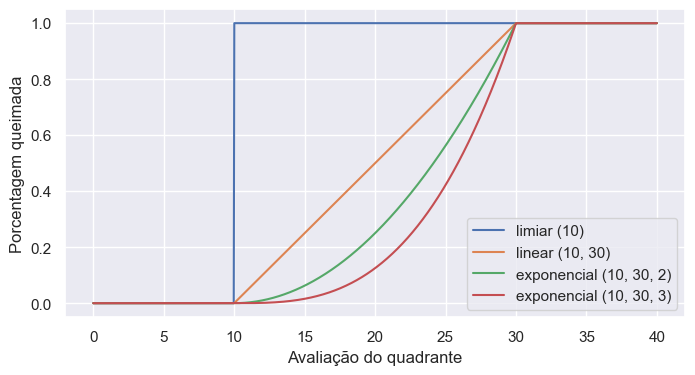
\includegraphics[width=25em]{eval_func_built_in}
    \end{center}
    \legend{Fonte: O Autor}
    \label{fig:eval_func_built_in}
\end{figure}

A Figura \ref{fig:aplicacao_funcoes_built_in} ilustra claramente como diferentes funções e parâmetros podem afetar significativamente os resultados na determinação da área queimada. Cada gráfico mostra a área queimada total calculada usando a função de área queimada indicada no título. Observa-se que a função limiar identifica mais áreas como queimadas, pois trata de forma igual os quadrantes com diferentes níveis de intensidade. No entanto, as funções exponenciais parecem mais próximas da realidade, já que consideram apenas uma porcentagem da área dos quadrantes próximos aos agrupamentos de alta intensidade como queimados. \par

\begin{figure}[H]
    \caption{Exemplo da aplicação das funções embutidas.}
    \begin{center}
        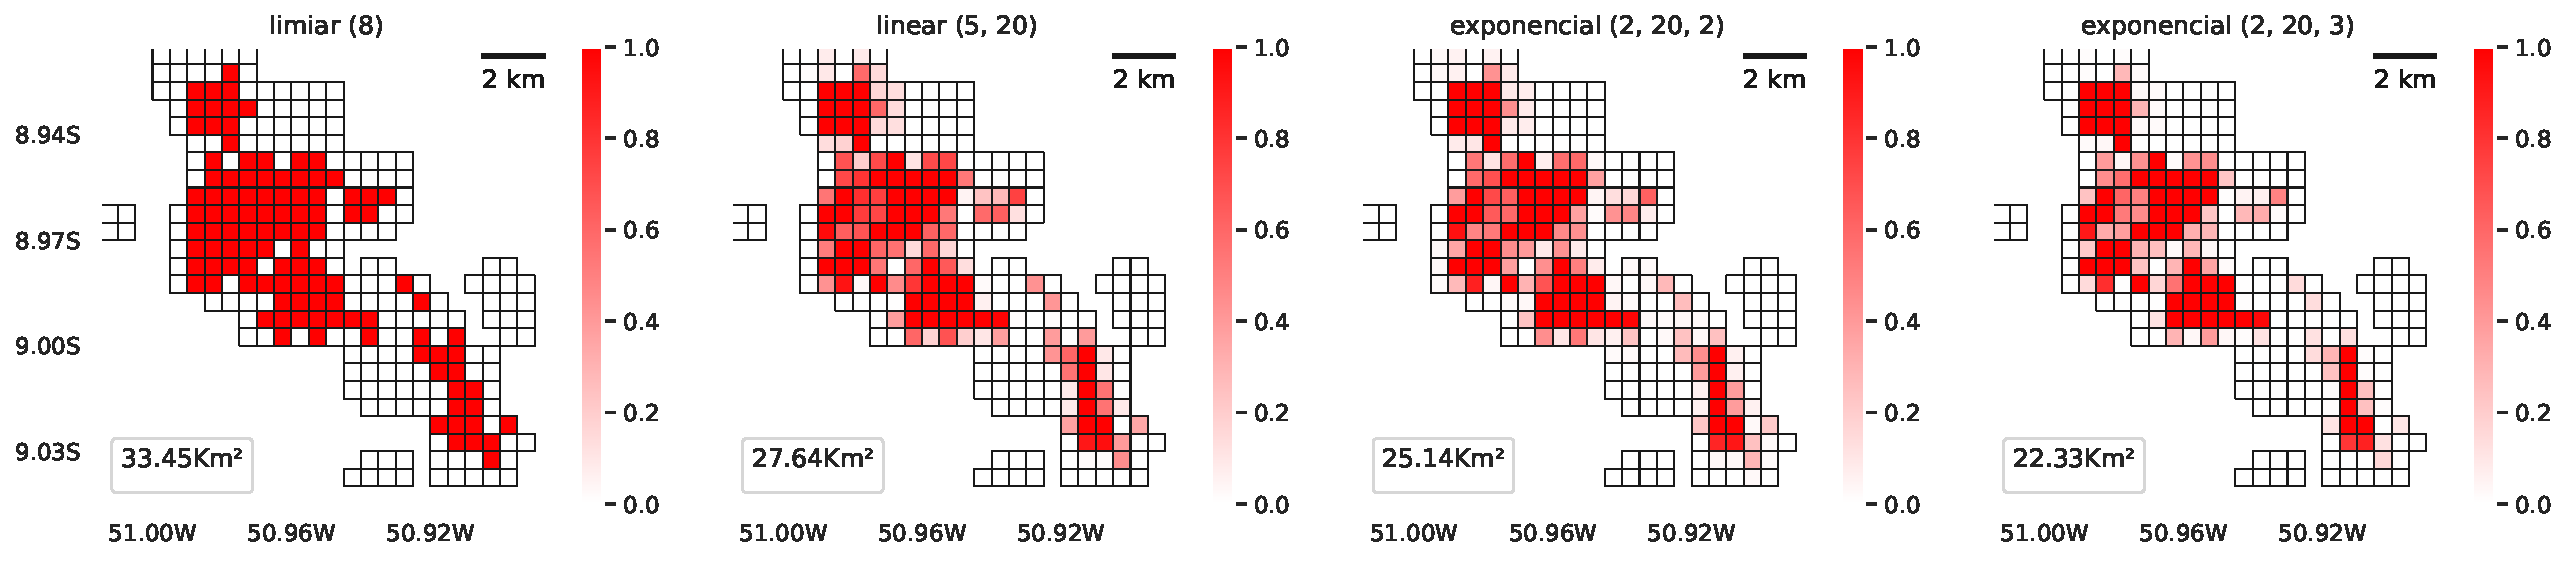
\includegraphics[width=35em]{aplicacao_funcoes_built_in}
    \end{center}
    \legend{Fonte: O Autor}
    \label{fig:aplicacao_funcoes_built_in}
\end{figure}

\chapter{Implementação do método}

Após a formalização do método de forma abstrata, esse capítulo descorre sobre a implementação de fato do método. Primeiro está discutido como os dados do DBQueimadas foram coletados da base de forma automatizada. Em seguida, descorre-se sobre a implementação do método ....

\section{Coleta dos dados}

Uma parte fundamental do processo foi coletar os dados do site DBQueimadas, que é a fonte primária usada para cálculo das áreas queimadas. Para exportar os dados usando o navegador, é necessário preencher um formulário com os campos de data inicial, data final e um endereço de e-mail, com intervalo de tempo máximo um ano para cada pedido. Também é possível aplicar filtros ainda mais específicos, como continente, país, estado, município, satélite, bioma e unidades de conservação/terras indígenas. Após clicar em "Exportar", uma mensagem contendo um link de download é enviada para o e-mail informado, e o arquivo disponibilizado é um CSV compactado em formato zip.

Embora o site tenha boa usabilidade, seria impraticável baixar todos os dados do Brasil manualmente sem sobrecarregar os servidores no INPE. Por isso, foi necessário entender como a solicitação dos dados era processada pelo site e, assim, automatizar o download. Foi identificado que o site faz uma requisição GET para a API do DBQueimadas, localizada em \url{https://queimadas.dgi.inpe.br/queimadas/exportacaobdq/exportar}, passando os parâmetros  codificados em JSON da URL, incluindo os filtros, e-mail e formato de arquivo desejado. Um exemplo de uso dessa API por meio de uma chamada CURL pode ser encontrado no \ref{anexo:usoApiInpe}.

Para automatizar o processo, desenvolvemos um script em Python que solicitava os dados de cada 30 dias, totalizando 300 requisições desde 1998 até 2022. Para não sobrecarregar os servidores do INPE, adicionamos uma espera de um minuto entre as requisições. Além disso, implementamos um sistema de registro de requisições em arquivo, que armazenou o estado de cada uma delas, evitando requisições duplicadas e possibilitando a retentativa das requisições que falharam por algum motivo. O programa foi considerado concluído apenas quando todas as requisições contidas no registro estavam marcadas como concluídas.

Para concluir o processo, ainda era necessário fazer o download do arquivo por meio do link enviado por e-mail. Utilizamos o Google Scripts, uma ferramenta que possibilita escrever programas simples, utilizando uma linguagem semelhante a JavaScript, com integração aos serviços do Google (como o Gmail). O script era executado com um intervalo de dois minutos, varrendo todos os e-mails novos provenientes do DBQueimadas. Com ele, foi possível extrair o link de cada mensagem e, finalmente, salvar o arquivo de forma automatizada. 

Os dois scripts trabalharam de forma concomitantemente, funcionando como uma espécie de produtor e consumidor distribuído. Enquanto um requisitava os dados para do INPE, o outro vasculhava os e-mails e salvava o arquivo em uma pasta específica. Quando o primeiro script identificava (por meio do nome do arquivo) que a resposta já estava salva, marcava a requisição como concluída no registro. Caso uma requisição permanecesse por mais de 30 minutos no estado pendente, o script fazia uma nova solicitação aos servidores do INPE.

Todo o processo de investigação e recuperação dos dados levou cerca de uma semana. Todos os arquivos baixados ocupam pouco mais de 4 gigabytes de armazenamento em disco e, juntos, somam exatamente 43.782.758 linhas. Ao final, eles foram recompactados em um único arquivo zip (450 megabytes) que está disponível para download em \url{https://bit.ly/3IgHIXH}, independentemente dos servidores do INPE.

Também foi utilizado os dados públicos territoriais do Brasil provenientes do Instituto Brasileiro de Geografia e Estatística (IBGE) para gerar gráficos delimitados em municípios, unidades federativas e biomas. O processo de aquisição desses arquivos se deu diretamente no site do IBGE. Todos os arquivos baixados estão no formato Shapefile, que é o formato responsável por armazenar dados vetoriais geográficos.


\section{Implementação do método}

Para toda a implementação e análise dos dados, foram utilizadas diversas ferramentas do ecossistema Python para Data Science, tais como NumPy, Pandas e Matplotlib. Além disso, foram empregadas bibliotecas específicas para análise de dados geográficos, como GeoPandas, Pysal, Xarray e Shapely. Para garantir a reprodutibilidade das execuções e a organização do código, foi adotado o Jupyter Notebook. Todos o código e demais artefatos gerados durante o projeto podem ser encontrados em \url{https://github.com/josebraz/INPE-Queimadas}, disponibilizados sob a licença MIT. \par

A biblioteca GeoPandas, amplamente utilizada na implementação, é uma extensão do Pandas que adiciona uma coluna especial chamada 'geometry'. Essa coluna permite armazenar as coordenadas e o formato dos dados em um sistema de coordenadas pré-definido. Além disso, o GeoPandas integra-se à biblioteca Shapely, que é usada para realizar cálculos e operações em estruturas geométricas espaciais. Com o uso dessas bibliotecas, é possível executar operações avançadas da teoria dos conjuntos em elementos geométricos, como união, interseção, diferença, entre outras, além de calcular a área de qualquer polígono que represente uma área no espaço. \par

O GeoPandas também oferece suporte à operação de junção espacial (spatial join) de forma otimizada. O spatial join permite combinar diferentes conjuntos de dados com base em sua relação espacial, de maneira semelhante a uma junção em um banco de dados, porém levando em consideração a proximidade geográfica. É possível utilizar diferentes critérios de proximidade geográfica, como verificar se um ponto está dentro de um polígono ou determinar a interseção entre dois polígonos. No contexto da implementação, o spatial join é utilizado para obter todas as medições que intersectam cada quadrante (interseção entre dois polígonos), que é a principal informação usada para avaliar um quadrante. \par

Após a coleta de dados mencionada anteriormente, os dados foram carregados no Python e algumas otimizações nas estruturas foram realizadas. Os 300 arquivos das queimadas foram lidos pelo Pandas e concatenados em um único DataFrame. Foi necessário converter o fuso horário das datas, que estavam no formato UTC, para o fuso horário de Brasília, a fim de facilitar a compreensão dos gráficos para os usuários brasileiros. Além disso, as colunas de texto, como município, estado, país e satélite, foram convertidas em categorias, que são uma forma de enumeração disponível no Pandas. Essa conversão ajudou a reduzir o consumo de memória, uma vez que muitos valores repetidos ocorriam nessas colunas, ocupando 2 Gb em mémoria. \par

Para otimizar o processamento e a leitura dos dados, também foi utilizada a biblioteca Dask especializada no processamento paralelo e distribuído. Essa biblioteca oferece a capacidade de criar clusters locais ou se conectar a clusters remotos, permitindo o envio de tarefas completas para serem processadas pelo cluster. Além disso, o Dask possibilita a leitura dos arquivos de forma paralela, o que resulta em uma redução significativa no tempo de carregamento dos dados. Após o carregamento completo do DataFrame a partir dos arquivos CSV originais durante a primeira execução, foi criado um arquivo no formato H5 que contém os mesmos dados, mas com uma estrutura otimizada para permitir uma leitura mais rápida. Nas execuções subsequentes do programa, ao invés de carregar novamente os arquivos CSV, o programa fará a leitura desse único arquivo H5, resultando em um carregamento ainda mais rápido dos dados.  \par

Durante o pré-processamento dos dados, foram identificadas regras de nomenclatura especiais para alguns satélites. No caso dos satélites AQUA (AQUA\_M-T e AQUA\_M-M) e TERRA (TERRA\_M-T e TERRA\_M-M), a última letra indica o período do dia em que ocorreu a passagem do satélite, sendo "M" para Manhã e "T" para Tarde. Outros satélites, como Suomi NPP, NOAA-19, NOAA-18, NOAA-16, NOAA-15 e NOAA-12, podem apresentar a última letra do nome como "D" para Diurno. Com base nessa compreensão das regras de nomenclatura, foi possível criar uma nova coluna que fornece o nome simplificado dos satélites, facilitando algumas análises. Em comparação com a coluna original dos satélites, que tinha 32 valores possíveis, a nova coluna contém apenas 22 valores possíveis. Para cada satélite, foi escolhida uma cor única, conforme apresentado na Figura \ref{fig:cores_satelites}, que é utilizada em todos os gráficos apresentados neste documento. \par

\begin{figure}[H]
    \caption{Cores escolhidas para cada satélite.}
    \begin{center}
        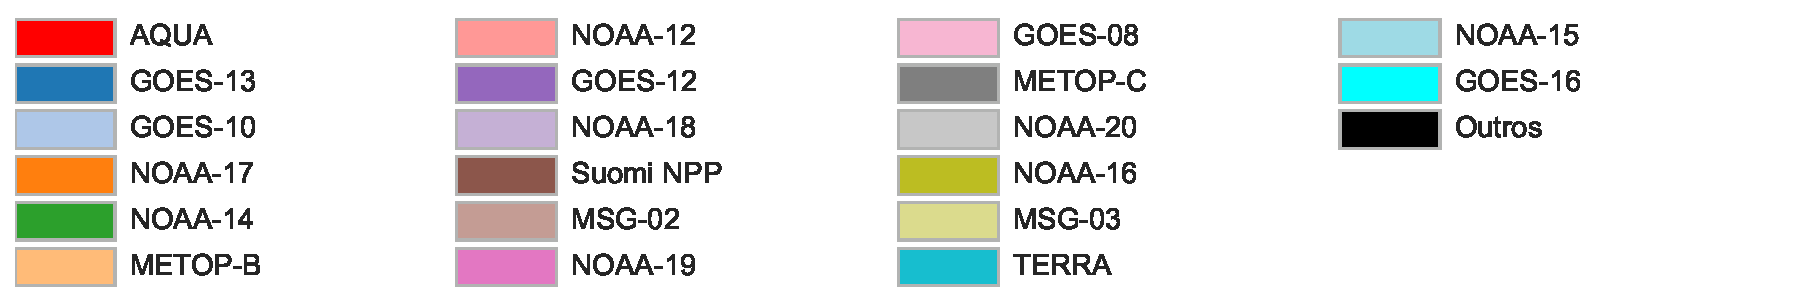
\includegraphics[width=35em]{cores_satelites}
    \end{center}
    \legend{Fonte: O Autor}
    \label{fig:cores_satelites}
\end{figure}


.... removido satélites ATSR .... removido satélites TRMM



....

A implementação das áreas dos focos, chamado de medições, usou os dados de satlélites de forma fixa no código (hardcoded). Apesar de exister bibliotecas especializadas em cálculos de órbitas de satélite, como a Orbital, essa abordagem foi escolhida a fim de evitar a necessidade de internet para execução do programa e simplificar o código. \par

Para simplificar e otimizar a implementação da parte das áreas dos focos, foi\par

------

A separação em quadrantes também foi planejada para melhorar o desempenho do processamento. Ao dividir o problema em partes menores, é possível resolver cada uma de forma paralela, pois as avaliações dos quadrantes são independentes entre si. Além disso, a separação em quadrantes otimiza ainda mais o processamento da junção espacial, que se beneficia quando os quadrantes para a interseção não são muito grandes. No entanto, é importante considerar que quanto maior o quadrante utilizado, menos avaliações são necessárias, mas a precisão da área queimada também é reduzida. Como se trata de um espaço bidimensional, a complexidade computacional da avaliação em relação à quantidade de quadrantes é $O(n^2)$. \par

\begin{figure}[H]
    \caption{Diferença da avaliação para diferentes tamanhos de quadrantes.}
    \begin{center}
        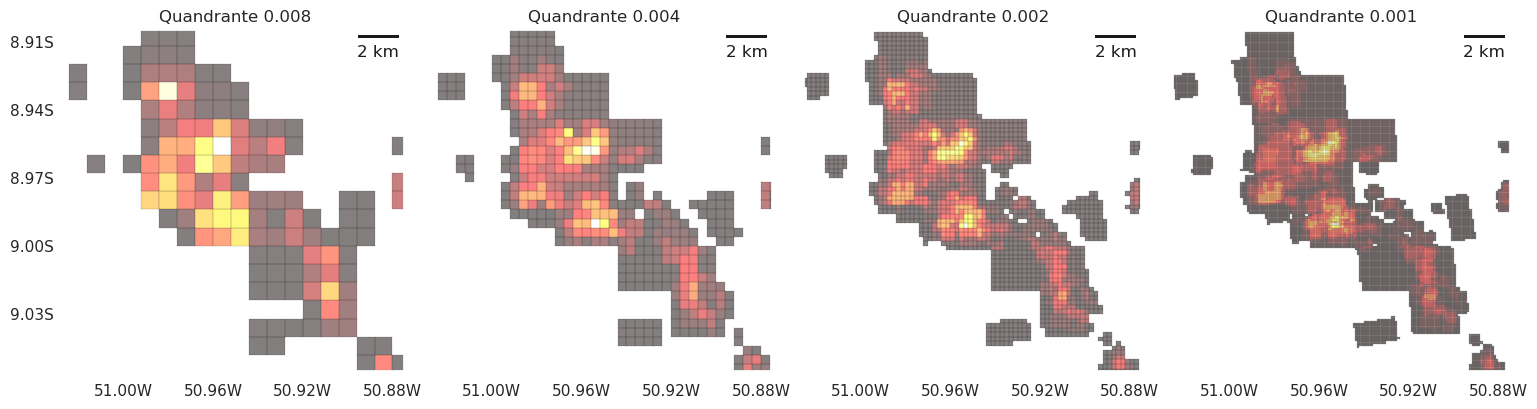
\includegraphics[width=35em]{diferenca_entre_quadrantes}
    \end{center}
    \legend{Fonte: O Autor}
    \label{fig:diferenca_entre_quadrantes}
\end{figure}

Com base em experimentos, foi constatado que o uso de quadrantes muito pequenos (com menos de 0,002 graus quadrados) não aumentam significativamente a precisão dos resultados e tornam a execução muito mais demorada.



%%%%%%%%%%%%%%%%%%%%%%%%%%%%%%%%%%%%%%%%%%%%%%%%%%%%%%%%%%%%%%%%%%%%%%%%%%%%%%%

\chapter{Resultados e Discussão}
\label{chp:resultados_discussão}

\section{Aplicações do método}

O método em sí é geral para qualquer entrada de focos de satélites, e retorna no final polígonos representando áreas geográficas associadas a um valor que indica a área queimada dentro desse polígono. Variando a entrada do método e o agrupamento dos resultados preliminares, pode-se obter diferentes resultados finais. \par


%%%%%%%%%%%%%%%%%%%%%%%%%%%%%%%%%%%%%%%%%%%%%%%%%%%%%%%%%%%%%%%%%%%%%%%%%%%%%%%

\chapter{Considerações Finais}

%%%%%%%%%%%%%%%%%%%%%%%%%%%%%%%%%%%%%%%%%%%%%%%%%%%%%%%%%%%%%%%%%%%%%%%%%%%%%%%


\bibliographystyle{abntex2-alf}
\bibliography{biblio}

\end{document}
